
En esta sección intentamos validar que el habla sintetizada por los modelos generados realmente puede ser identificada como perteneciente a personas de habla inglesa, y al mismo tiempo evaluar sus grados de inteligibilidad. Para eso se condujo una encuesta perceptual donde a cada participante se le presentó una oración sintetizada con distintos grados de mezcla de español e inglés y se le pidió que la transcribiera y que intentara identificar la nacionalidad del hablante. 

La encuesta se realizó a través de Internet, con el mismo set de instrucciones para todos los participantes y pidiendo como requisito la utilización de auriculares. Cada participante podía contestar un máximo de $5$ veces, presentándoles siempre oraciones distintas.

Nos propusimos como objetivo conseguir $5$ respuestas para cada uno de los $50$ audios sintetizados, momento en el cual se cerró la posibilidad de contestar. Se llevó a cabo desde el $18$ de octubre de $2017$ hasta el primero de diciembre del mismo año, tiempo durante el cual fue publicitada en distintas redes sociales y listas de emails de la facultad.

Con el objetivo de no influir en las respuestas de los participantes, se procuró darles la información mínima indispensable para completar la encuesta. Por este motivo, en ningún momento de la encuesta se especifica el objetivo real de la misma. Con la intención de homogeneizar la muestra, fue requisito obligatorio utilizar auriculares para la encuesta. También se le pidió a cada participante que la realizara en un lugar silencioso y tranquilo.

A continuación, describimos la forma en que se construyeron los audios usados en esta evaluación y la interfaz de la encuesta. Luego mostramos los datos demográficos  obtenidos. Más adelante, continuamos con un análisis exhaustivo de inteligibilidad y origen atribuido a las oraciones.
Por último, para evaluar la hipótesis original, compondremos estos dos ejes para dilucidar el grado de validez de los resultados.

\section{Audios sintetizados}

Para evitar que el participante pudiera deducir las palabras a partir de las palabras vecinas, las mismas fueron generadas de manera \textit{semánticamente impredecible}. Esto significa que a partir de una lista de sustantivos, adjetivos, determinantes y verbos se generaron oraciones de manera aleatoria con la siguiente estructura:

$$\textnormal{\textit{Determinante Adjetivo Sustantivo Verbo Determinante Sustantivo}}$$

Luego, para asegurarnos de estar cubriendo todos los posibles fonos del castellano, las oraciones fueron modificadas para ser fonéticamente balanceadas. Esto significa que incluimos entre cinco y diez veces cada fono perteneciente a una consonante (del castellano) y al menos veinte veces cada fono perteneciente a una vocal.

Los oraciones generadas fueron:

\begin{itemize}
\item Oración 1: Mi montaña aguileña recorrió la esquina
\item Oración 2: Aquel fuerte vidrio prefirió aquel botón
\item Oración 3: Este enjoyado juez comprará nuestro corchete
\item Oración 4: Tu estrecho posavasos gritó la fechoría
\item Oración 5: Nuestro nublado tigre concluyó a este chupetín
\item Oración 6: Su profundo riñón apoyó a Julio
\item Oración 7: El frío churrasco oyó lo de Polonia
\item Oración 8: Las acongojadas cotorras sonrieron a mi círculo
\item Oración 9: Ese gruñón perro prometió a esos cuñados
\item Oración 10: El nudillo argentino perdió su vaso
\end{itemize}

Para cada una de estas diez oraciones se varió el nivel de mezcla entre $30\%$ de inglés + $70\%$ castellano hasta $70\%$ de inglés + $30\%$ de castellano, con $10\%$ de incremento. De esta manera, para cada oración hay $5$ mezclas diferentes, lo que hace un total de $50$ audios sintetizados diferentes.

\section{Interfaz}\label{interfaz}

En esta sección se presenta la interfaz utilizada para realizar la encuesta junto con las decisiones de diseño más relevantes. En la Figura \ref{personalData} se presenta la página con la que todos los participantes fueron recibidos. A fin de conocer de manera general la demografía encuestada, a cada participante se le pidió que indicara el rango correspondiente a su edad, yendo desde $18$ a $25$, $26$ a $35$, y así de diez en diez.

\begin{figure}[htp]
\begin{center}
\fbox{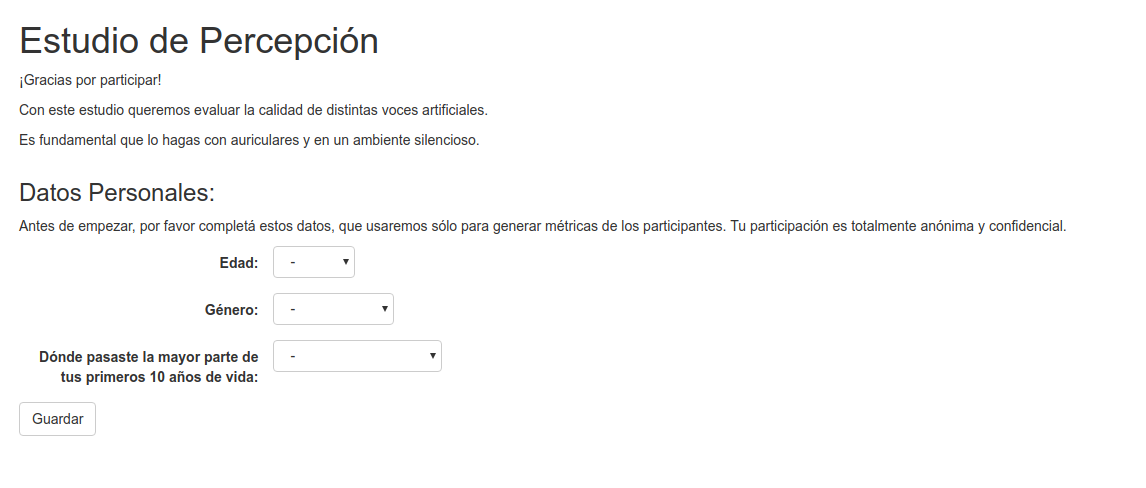
\includegraphics[scale=0.6]{estudio_online/estudio1.png}}
\end{center}
\caption{Primera pantalla de la encuesta, en la cual se recaban datos personales}
\label{personalData}
\end{figure}

Se le pidió, además, que indicara su género: ``masculino'', ``femenino'', ``otro'', ``no contesta'' y la provincia donde pasó la mayor parte de sus primeros diez años de vida. Consideramos que estos datos son importantes para el estudio ya que dependiendo de ellos los resultados variarán indefectiblemente. Por ejemplo la transcripción que obtendremos de un participante de $50$ años de Capital Federal será distinta a la de alguien de $18$ años de Córdoba. El diferente uso de los alofonos, modismos y variantes prosódicas y capacidades auditivas jugarán un papel importante en la interpretación de la oración y la apreciación del origen del hablante.

\begin{figure}
\begin{center}
\fbox{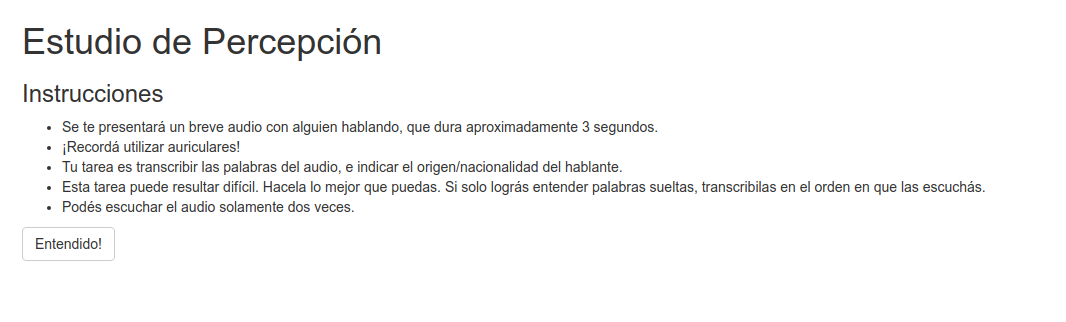
\includegraphics[scale=0.6]{estudio_online/estudio2.png}}
\end{center}
\caption{Pantalla con las instrucciones de la encuesta}
\label{instrucciones}
\end{figure}

Como puede verse en la Figura \ref{instrucciones}, una vez completados estos datos, a cada participante se le presentó otra vista con las instrucciones específicas para completar la encuesta. Una vez presionado el botón de ``Entendido!'' se les presentó el primer audio, que podían escuchar un máximo de $2$ veces, una caja de texto libre donde ingresar la transcripción del mismo y una caja de texto libre donde podían escribir cual consideraban que era el origen de la nacionalidad correspondiente a la voz, como puede apreciarse en la Figura \ref{transcripcion}.

\begin{figure}
\begin{center}
\fbox{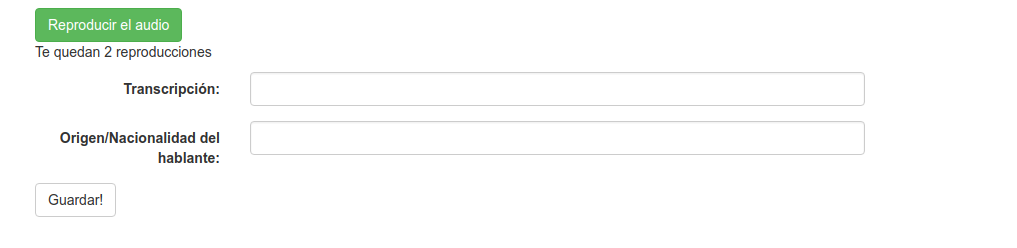
\includegraphics[scale=0.6]{estudio_online/estudio3.png}}
\end{center}
\caption{Pantalla de transcripción}
\label{transcripcion}
\end{figure}

Una vez guardada la respuesta, se le preguntó si quería continuar transcribiendo otro audio. En caso de haber completado cinco audios, se le mostró un mensaje indicando que ya podía cerrar la encuesta:

\begin{center}
\fbox{
¡Muchas gracias por tu participación! Ya podés cerrar la ventana del navegador.}
\end{center}
